
\documentclass{beamer}
\usetheme{Singapore}
\usecolortheme[dark,accent=blue]{solarized}
\setbeamertemplate{navigation symbols}{\insertframenumber}
\setbeamercolor{navigation symbols}{fg = solarizedAccent}
\setbeamerfont{navigation symbols}{size = \tiny}

\usepackage{hyperref, tikz}
\usetikzlibrary{arrows.meta, shapes.geometric}
\tikzset{>={To[length=3mm,width=3mm]}}

\title{Winning baseball games by\\solving statistics puzzles}
\author{Scott Powers}
\date{ICSDS 2025}
\begin{document}

  \begin{frame}
      \maketitle
      \vfill\hfill
\includegraphics[width = 4cm]{../../assets/rice_logo_white.png}
  \end{frame}
  
  \begin{frame}{Outline}
    \begin{enumerate}
      \item Pickoff Game Theory
      \begin{itemize}
        \item Linear mixed-effects model (LMM)
        \item Markov decision process (MDP)
      \end{itemize}
      \item Predictive Pitch Score
      \begin{itemize}
        \item Bayesian hierarchical model
        \item Supervised learning
      \end{itemize}
      \item Swinging, Fast and Slow
      \begin{itemize}
        \item Bayesian hierarchical model (skew-normal!)
        \item Instrumental variables regression
      \end{itemize}
    \end{enumerate}
  \end{frame}

  \begin{frame}
    \Large Part I: Pickoff Game Theory \normalsize\\
    \vfill
    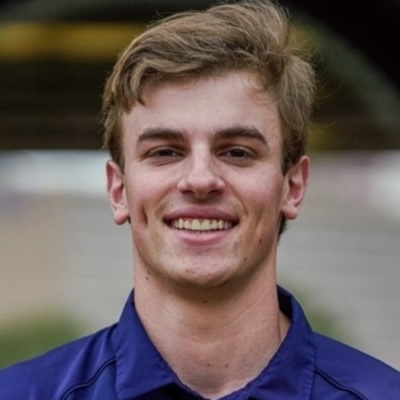
\includegraphics[height=0.5in]{images/collaborators/hahn.jpg}
    \alert{Jacob Hahn}, Rice University $\rightarrow$ Chicago Cubs\\
    ~\\
    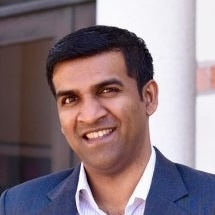
\includegraphics[height=0.5in]{images/collaborators/pai.jpg}
    \alert{Mallesh Pai}, Rice University\\
    ~\\
    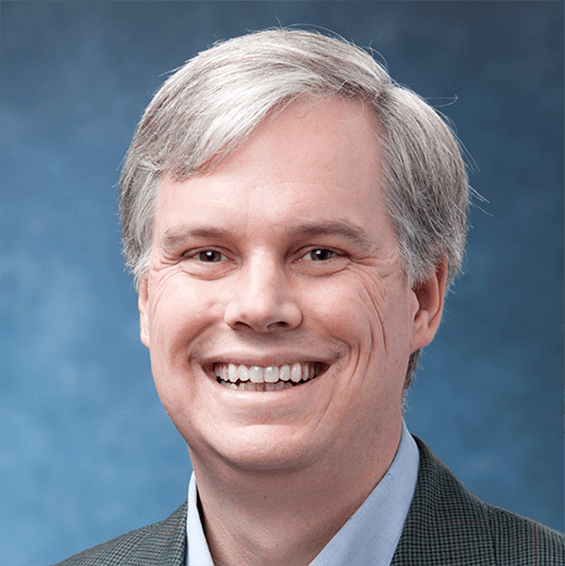
\includegraphics[height=0.5in]{images/collaborators/schaefer.png}
    \alert{Andrew Schaefer}, Rice University\\
    ~\\
    Working paper:\\
    \small Hahn J, Powers S, Pai M, Schaefer A ``The Two-Foot Rule: A game theoretic analysis of the pickoff limit in Major League Baseball''
  \end{frame}

  \begin{frame}{Background}
    \centering
    
\includegraphics[width = 0.8\textwidth]{images/cat_and_mouse.jpg}
    \begin{itemize}
      \item In 2023, MLB limited the pitcher to 3 pickoff attempts
      \item After 3 failed pickoffs, the runner advances automatically
    \end{itemize}
  \end{frame}

  \begin{frame}{The Puzzle}
    If you are the runner, how much should you extend your lead after each pickoff attempt?\\
    \vfill
    Data: pitch-by-pitch lead distance (player tracking) from MLB*\\
    \vfill
    \footnotesize \it *Major League Baseball trademarks and copyrights are used with permission of MLB Advanced Media, L.P. All rights reserved.
  \end{frame}

  \begin{frame}{Our Approach}
    Step 1: Estimate the effect of lead distance\\
    \begin{itemize}
      \item Linear mixed-effects models (LMMs) for probabilities of pickoff attempt, pickoff success, stolen base success
      \item Fixed effects: lead distance, disengagements, outs, count, catcher arm strength, runner sprint speed
      \item Random effects: pitcher, catcher, runner identities
    \end{itemize}
    ~\\
    Step 2: Solve for the optimal lead distance\\
    \begin{itemize}
      \item Markov decision process (MDP) to model an inning
      \item State space: disengagements, bases occupied, outs, count
      \item Action space: lead distance
      \item Reward function: runs scored
    \end{itemize}
  \end{frame}

  \begin{frame}{Results: Pickoff Attempt and Success Probability}
    \centering
    \includegraphics[width = 0.45\textwidth]{figures/prob_po_attempt_dark.pdf}
    \hfill
    \includegraphics[width = 0.45\textwidth]{figures/prob_po_success_dark.pdf}
  \end{frame}

  \begin{frame}{Results: Stolen Base Success Probability}
    \centering
    \includegraphics[width = \textwidth]{figures/prob_sb_success_dark.pdf}
  \end{frame}

  \begin{frame}{Results: Runner and Catcher Effects}
    \centering
    \includegraphics[width = 0.45\textwidth]{figures/effect_runner_dark.pdf}
    \hfill
    \includegraphics[width = 0.45\textwidth]{figures/effect_catcher_dark.pdf}
  \end{frame}

  \begin{frame}{Results: Optimal Lead Distance}
    \begin{center}
      \begin{tabular}{c|cc|c}
 & \multicolumn{2}{c|}{Average Lead} & Actual Exceeds \\
Disengagements & Actual & Recommended & Recommendation \\
% latex table generated in R 4.5.0 by xtable 1.8-4 package
% Mon Jun 23 17:25:30 2025
  \hline
0 & 9.5 & 10.3 & 31.1\% \\ 
  1 & 10.2 & 11.7 & 12.4\% \\ 
  2 & 10.8 & 14.1 & 1.0\% \\ 
\end{tabular}

    \end{center}
    \vfill
    Additional results in paper:
    \begin{itemize}
      \item What if you are not an average runner?
      \item What if the pitcher has agency? (game theory)
    \end{itemize}
  \end{frame}

  \begin{frame}
    \Large Part II: Predictive Pitch Score \normalsize\\
    \vfill
    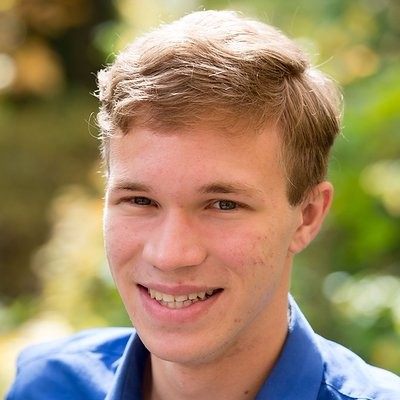
\includegraphics[height=0.5in]{images/collaborators/iglesias.jpg}
    \alert{Vicente Iglesias}, Susquehanna International Group\\
    ~\\
    Working paper:\\
    \small Powers S, Iglesias V ``Pitch trajectory density estimation for predicting future outcomes''
  \end{frame}

  \begin{frame}{Background}
    \begin{center}
      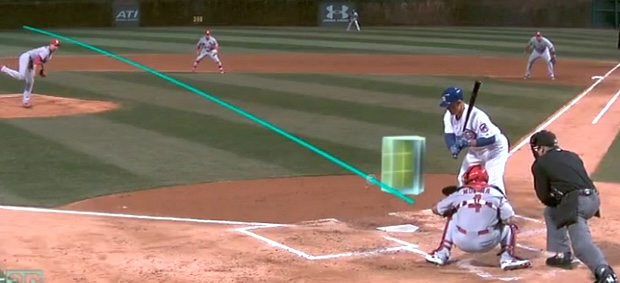
\includegraphics[width = 0.8\textwidth]{images/pitch_tracking.jpg}
    \end{center}
    \begin{itemize}
      \item Full pitch tracking data have been available for two decades
      \item Trajectory estimated as 3D quadratic function of time ($\in \mathbb{R}^9$)
      \item Standard practice: Evaluate pitchers based on trajectories
    \end{itemize}
  \end{frame}

  \begin{frame}{The Puzzle}
    \begin{columns}
      \begin{column}{0.5\textwidth}
        \centering
        $\mbox{Variable Importance}^1$\\
        \includegraphics[width = \textwidth]{figures/feature_importance_dark.pdf}
      \end{column}
      \begin{column}{0.5\textwidth}
        \centering
        $\mbox{Variable Reliability}^2$\\
        \includegraphics[width = \textwidth]{figures/feature_reliability_dark.pdf}
      \end{column}
    \end{columns}
    \scriptsize
    \vfill
    ${}^1$ fractional contribution of each feature's splits to gradient boosting pitch model\\
    ${}^2$ (between-pitcher variance) / (total variance); varies by pitch type (here: RHB FB)
  \end{frame}

  \begin{frame}{Why Supervised Learning Isn't Enough}
    \begin{columns}
      \begin{column}{0.4\columnwidth}
        \centering
        {\bf Supervised Learning}\\
        ~\\
        \begin{tabular}{ccc}
          Pitch &               & Outcome\\
          $x_1$ & $\rightarrow$ & $y_1$\\
          $x_2$ & $\rightarrow$ & $y_2$\\
          $x_3$ & $\rightarrow$ & $y_3$\\
                & ...           &      \\
          $x_n$ & $\rightarrow$ & $y_n$\\
          \\
          \\
          \\
          $x^*$ & $\rightarrow$ & $\hat y$\\
        \end{tabular}
      \end{column}
      \begin{column}{0.6\columnwidth}
        \centering
        {\bf Our Problem}\\
        ~\\
        \begin{tabular}{cccc}
          Pitcher & Pitch &               & Outcome\\
          A       & $x_1$ & $\rightarrow$ & $y_1$\\
          A       & $x_2$ & $\rightarrow$ & $y_2$\\
          B       & $x_3$ & $\rightarrow$ & $y_3$\\
                  &       & ...           &      \\
          C       & $x_n$ & $\rightarrow$ & $y_n$\\
                  & \\
                  &       & $\searrow$    & {\color{solarizedRebase03} $\int\hat p(x)\hat f(x)$}\\
                  & \\
          A       &       &               & $\hat y$\\
        \end{tabular}
      \end{column}
    \end{columns}
  \end{frame}

  \begin{frame}{Why Supervised Learning Isn't Enough}
    \begin{columns}
      \begin{column}{0.4\columnwidth}
        \centering
        {\bf Supervised Learning}\\
        ~\\
        \begin{tabular}{ccc}
          Pitch &               & Outcome\\
          $x_1$ & $\rightarrow$ & $y_1$\\
          $x_2$ & $\rightarrow$ & $y_2$\\
          $x_3$ & $\rightarrow$ & $y_3$\\
                & ...           &      \\
          $x_n$ & $\rightarrow$ & $y_n$\\
          \\
          \\
          \\
          $x^*$ & $\rightarrow$ & $\hat y$\\
        \end{tabular}
      \end{column}
      \begin{column}{0.6\columnwidth}
        \centering
        \alert{\bf Our Approach}\\
        ~\\
        \begin{tabular}{cccc}
          Pitcher & Pitch &               & Outcome\\
          A       & $x_1$ & $\rightarrow$ & $y_1$\\
          A       & $x_2$ & $\rightarrow$ & $y_2$\\
          B       & $x_3$ & $\rightarrow$ & $y_3$\\
                  &       & ...           &      \\
          C       & $x_n$ & $\rightarrow$ & $y_n$\\
                  & \\
                  & \alert{$\downarrow$}\\
                  & \\
          A       & \alert{$\hat p(x)$} & \alert{$\rightarrow$} & \alert{$\int\hat p(x)\hat f(x)$}\\
        \end{tabular}
      \end{column}
    \end{columns}
  \end{frame}

  \begin{frame}{Our Approach}
    Step 1: Estimate trajectory distributions conditional on covariates\\
    \begin{itemize}
      \item Bayesian hierarchical model (9D MVN likelihood)
      \item Mean $\sim$ pitcher, context, pitcher $\times$ context
      \item Variance scaling $\sim$ pitcher, context
      \item Correlation $\sim$ pitcher
      \item Fit via maximum {\it a posteriori} (MAP) estimator
    \end{itemize}
    ~\\
    Step 2: Fit supervised learning model and integrate w.r.t. Step 1\\
    \begin{itemize}
      \item Gradient boosting
    \end{itemize}
  \end{frame}

  \begin{frame}{Results: Illustration of Estimated Distribution}{Dylan Cease Slider vs RHB}
    \vfill
    \centering
    
\includegraphics[height = 0.85\textheight]{figures/656302_SL_R_plate.png}
  \end{frame}

  \begin{frame}{Results: Predictive Performance}
    \centering
    
\includegraphics[width = \textwidth]{figures/cor_by_sample_size.pdf}
  \end{frame}

  \begin{frame}
    \Large Part III: Swinging, Fast and Slow \normalsize\\
    \vfill
    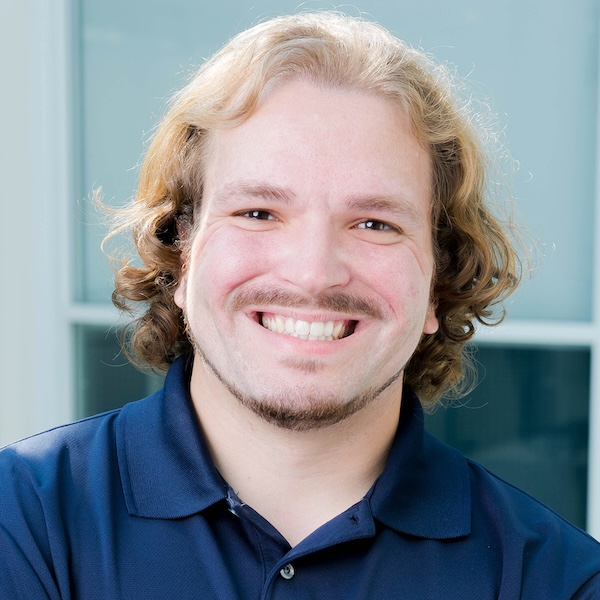
\includegraphics[height=0.5in]{images/collaborators/yurko.jpg}
    \alert{Ron Yurko}, Carnegie Mellon University\\
    ~\\
    Working paper:\\
    \small Powers S, Yurko R ``Swinging, Fast and Slow: Interpreting variation in baseball swing tracking metrics''
  \end{frame}

  \begin{frame}{Background}
    \begin{center}
      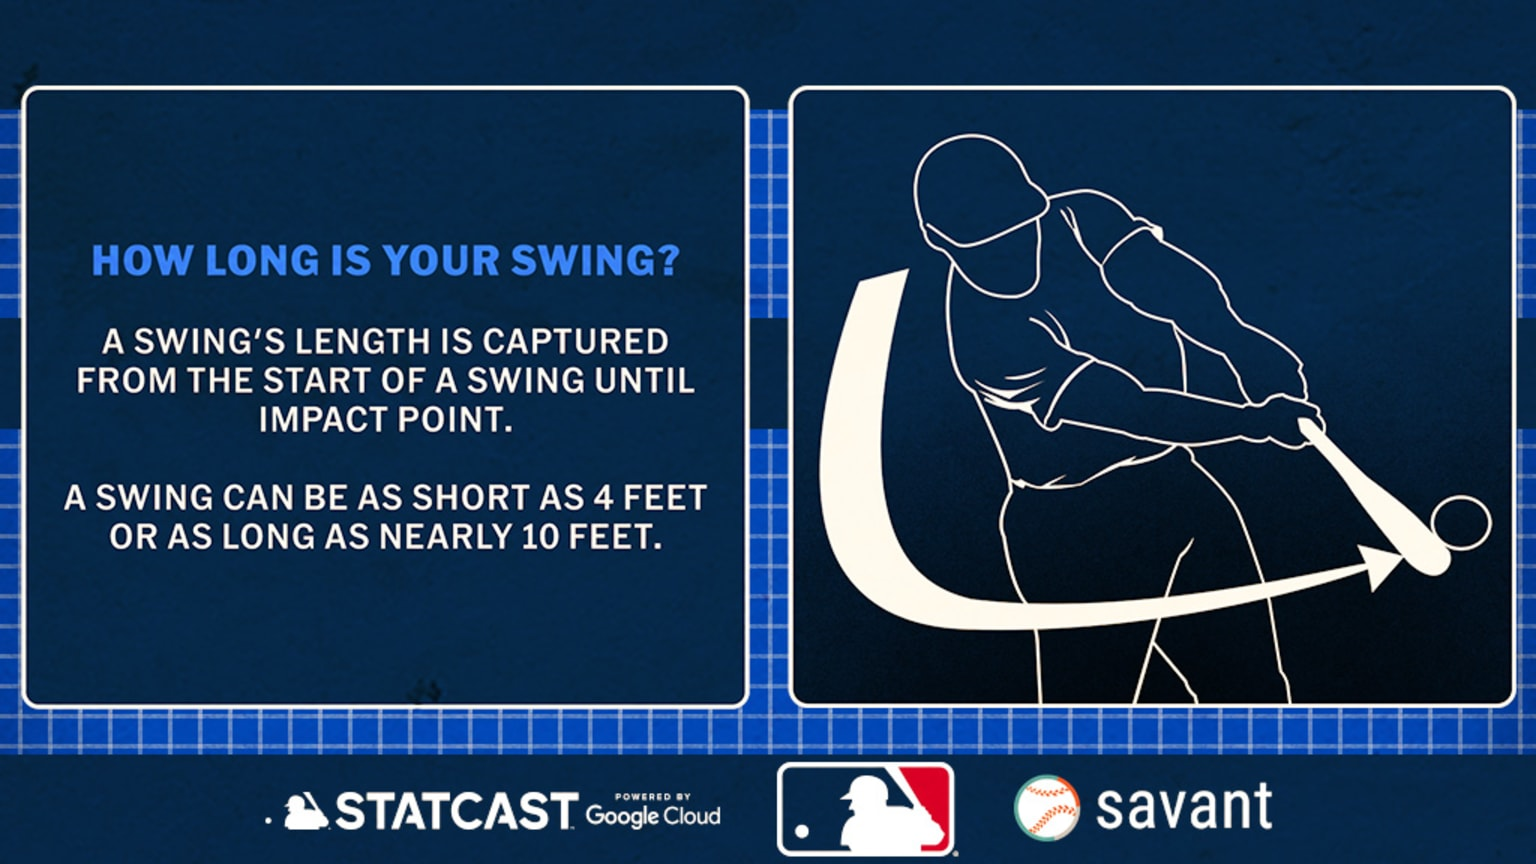
\includegraphics[width = 0.8\textwidth]{images/swing_length.jpg}
    \end{center}
    \begin{itemize}
      \item In May 2024, MLB released swing length and bat speed data
      \item Both are measured at contact (or at point nearest to contact)
    \end{itemize}
  \end{frame}

  \begin{frame}{The Puzzle}
    \begin{center}
      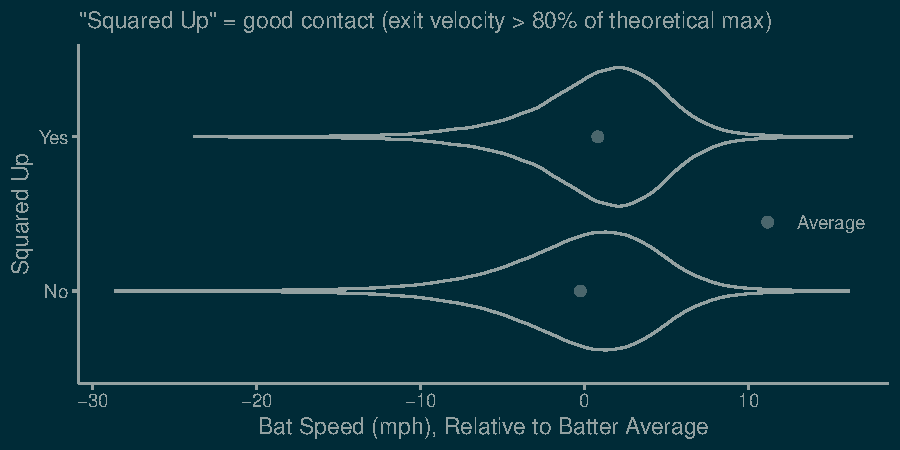
\includegraphics[width = \textwidth]{figures/counterintuitive.pdf}
    \end{center}
    \begin{itemize}
      \item How should batters modulate swing length and bat speed?
    \end{itemize}
  \end{frame}

  \begin{frame}{Challenge \#1: Measurement}
    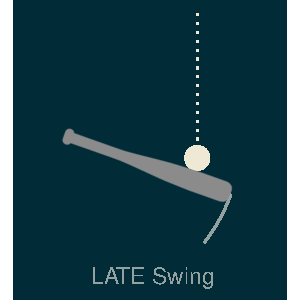
\includegraphics[width = 0.49\textwidth]{figures/swing_late.pdf}
    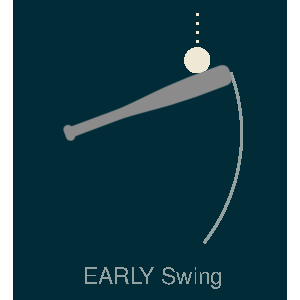
\includegraphics[width = 0.49\textwidth]{figures/swing_early.pdf}
    \begin{itemize}
      \item For \alert{identical} swings, timing determines point of measurement
      \item Swing length and bat speed are \alert{outcomes}, not purely process
    \end{itemize}
  \end{frame}

  \begin{frame}{Challenge \#2: Confounding}
    \begin{center}
      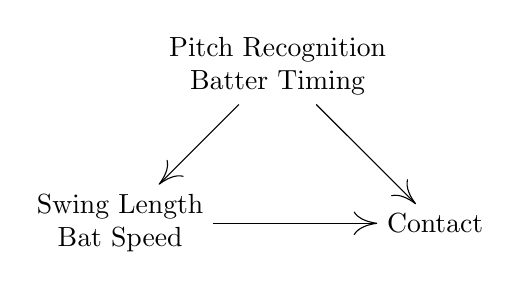
\begin{tikzpicture}[->, align = center]
        \node (confounders) at (2, 2) {Pitch Recognition \\ Batter Timing};
        \node (swing_metrics) at (0, 0) {Swing Length \\ Bat Speed};
        \node (contact) at (4, 0) {Contact};
        \draw (confounders) -- (swing_metrics);
        \draw (confounders) -- (contact);
        \draw (swing_metrics) -- (contact);
      \end{tikzpicture}
    \end{center}
  \end{frame}

  \begin{frame}{Our Approach}
    Step 1: Estimate batter intention\\
    \begin{itemize}
      \item Bayesian hierarchical model (skew-normal likelihood)
      \item Condition on successful contact against fastballs!
      \item Mean $\sim$ batter, count, location, batter $\times$ (count, location)
      \item Skew $\sim$ batter
    \end{itemize}
    ~\\
    Step 2: Estimate effect of batter intention\\
    \begin{itemize}
      \item Instrumental variable regression (instrument: count)
      \item Control for pitch difficulty using pitch outcome model (Part II)
      \item Response: contact (logistic reg.) and ``power'' (linear reg.)
    \end{itemize}
    ~\\
    Step 3: Value the tradeoff between contact and power
    \begin{itemize}
      \item Model the plate appearance as a Markov chain
    \end{itemize}
  \end{frame}

  \begin{frame}{Results: Batter $\times$ Count Interaction}
    \centering
    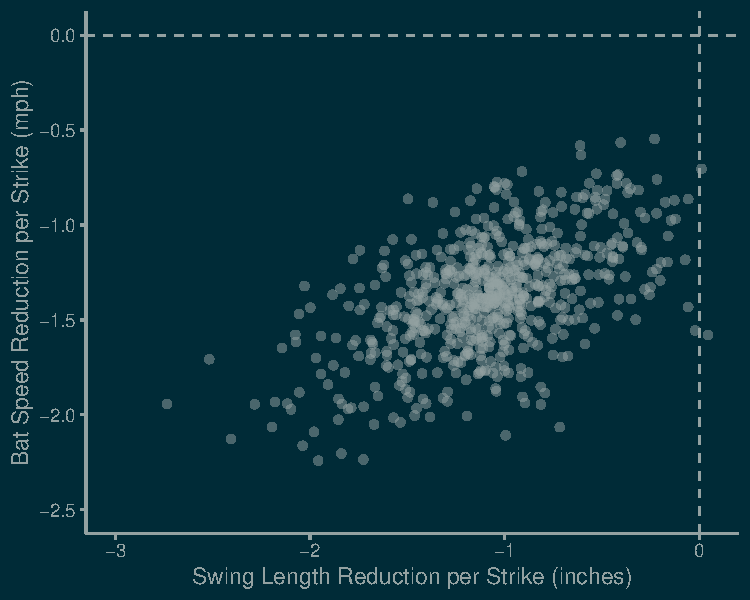
\includegraphics[height = 0.8\textheight]{figures/approach.pdf}
  \end{frame}

  \begin{frame}{Results: Causal Effect Estimates}
    \centering
    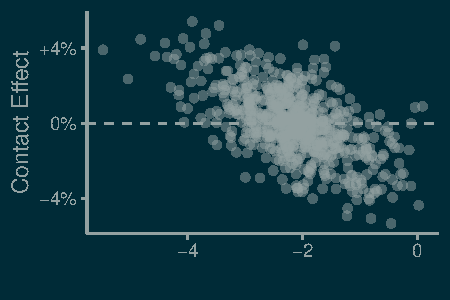
\includegraphics[width = 0.49\textwidth]{figures/swing_length_contact.pdf}
    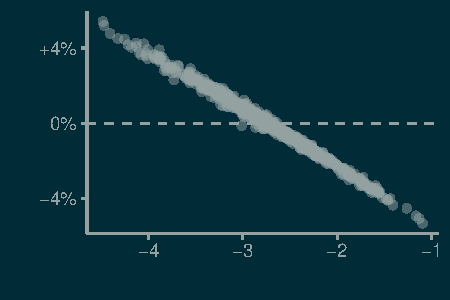
\includegraphics[width = 0.49\textwidth]{figures/bat_speed_contact.pdf}\\
    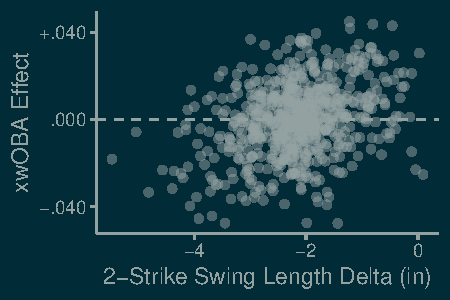
\includegraphics[width = 0.49\textwidth]{figures/swing_length_power.pdf}
    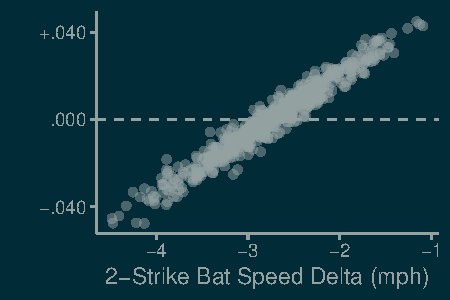
\includegraphics[width = 0.49\textwidth]{figures/bat_speed_power.pdf}
  \end{frame}

  \begin{frame}{Results: Contact-Power Tradeoff}
    \centering
    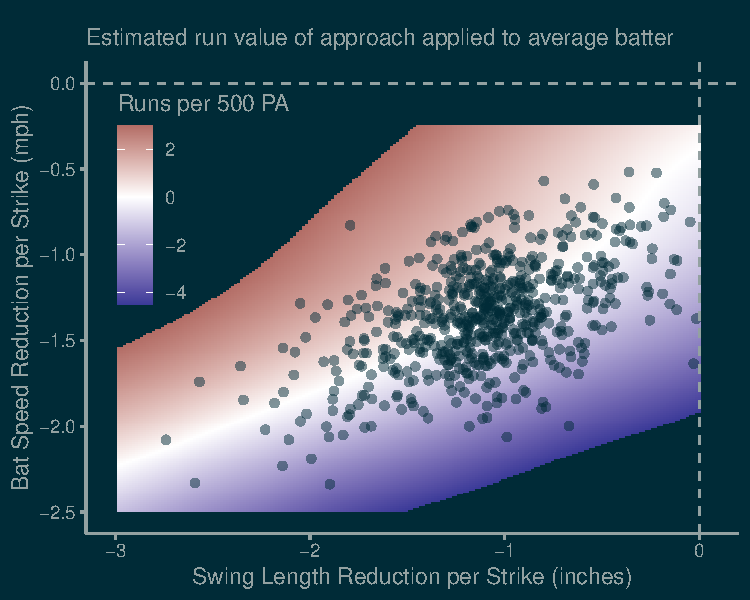
\includegraphics[height = 0.9\textheight]{figures/approach_run_value.pdf}
  \end{frame}

  \begin{frame}{Thank You!}
    \centering saberpowers.github.io
  \end{frame}

\end{document}
